% =====================================================================
\section{Kết quả}
% =====================================================================
 
\subsection{Hiệu năng trên ba tập}
 
\begin{table}[H]
\centering\small
\caption{Accuracy và macro-F1 của cấu hình cuối trên train (54\,000), validation (6\,000) và test (10\,000). In đậm: tốt nhất theo cột.}\label{tab:main}
\setlength{\tabcolsep}{4pt}
\begin{tabular}{@{}lcccccccc@{}}
\toprule
& \multicolumn{3}{c}{Accuracy} & \multicolumn{3}{c}{Macro-F1} & Khoảng cách & Dự đoán \\
\cmidrule(lr){2-4}\cmidrule(lr){5-7}
Mô hình & Train & Val & Test & Train & Val & Test & train$-$test & (ms/ảnh) \\
\midrule
Multinomial NB      & 0.8248 & 0.8210 & 0.8364 & 0.8235 & 0.8199 & 0.8349 & $-0.012$ & 0.007 \\
Logistic Regression & 0.9244 & 0.9167 & 0.9213 & 0.9234 & 0.9155 & 0.9201 & $\phantom{-}0.003$ & 0.002 \\
MLP 784-256-128-10  & \textbf{0.9998} & \textbf{0.9813} & \textbf{0.9809} & \textbf{0.9998} & \textbf{0.9813} & \textbf{0.9808} & $\phantom{-}0.019$ & 0.002 \\
Random Forest ($T{=}50$) & 0.9971 & 0.9622 & 0.9645 & 0.9971 & 0.9618 & 0.9642 & $\phantom{-}0.033$ & 0.206 \\
\bottomrule
\end{tabular}
\end{table}
 
Thứ hạng nhất quán trên cả ba tập: MLP $>$ Random Forest $>$ Logistic Regression $>$ Naive Bayes. Accuracy validation và test chênh nhau dưới 1.6 điểm phần trăm với mọi mô hình, cho thấy validation 6\,000 ảnh là thước đo đáng tin để chọn siêu tham số. Hai mô hình tuyến tính/sinh có train $\approx$ test (gần như không overfit, nhưng underfit); MLP và Random Forest gần như thuộc lòng tập train (99.7--99.98\%). Random Forest có OOB score 0.9549, thấp hơn accuracy validation 0.9622 khoảng 0.7 điểm, đúng kỳ vọng vì mỗi mẫu OOB chỉ được khoảng 37\% số cây bỏ phiếu.
 
\subsection{Đối chiếu với thư viện chuẩn}
 
\begin{table}[H]
\centering\small
\caption{Đối chiếu cài đặt tự viết với thư viện chuẩn trên tập validation.}\label{tab:sklearn}
\setlength{\tabcolsep}{4pt}
\begin{tabular}{@{}l l c c >{\raggedright\arraybackslash}p{4.1cm}@{}}
\toprule
Mô hình & Đối chiếu với & Tự cài & Thư viện & Tiêu chí / nhận xét \\
\midrule
Multinomial NB & sklearn \code{MultinomialNB} & 0.8210 & 0.8210 & $\log\theta$, $\log\pi$, xác suất khớp (\code{allclose}); dự đoán trùng 100\% \\
Logistic Regression & sklearn \code{LogisticRegression} & 0.9167 & 0.9183 & quy đổi $C=1/(n\lambda)$; chênh 0.16 điểm \\
MLP 784-128-10 & PyTorch (SGD momentum) & 0.9768 & 0.9775 & cùng kiến trúc, khởi tạo He; chênh 0.07 điểm \\
Random Forest ($T{=}50$) & sklearn \code{RandomForestClassifier} & 0.9622 & 0.9608 & cùng tham số; chênh 0.14 điểm \\
\bottomrule
\end{tabular}
\end{table}
 
Naive Bayes khớp tuyệt đối với scikit-learn (khi so trên \code{float64}). Ba mô hình còn lại có thành phần ngẫu nhiên hoặc bộ tối ưu khác nhau nên chỉ cần chênh lệch nhỏ; mọi chênh lệch đều dưới 0.2 điểm phần trăm, và Random Forest tự cài thậm chí nhỉnh hơn bản scikit-learn ở hạt giống này. Kết quả này xác nhận hai cài đặt của nhóm đúng về mặt thuật toán.
 
\subsection{Ảnh hưởng của siêu tham số}
 
\begin{figure}[H]
\centering
\begin{subfigure}[b]{0.36\textwidth}\centering
  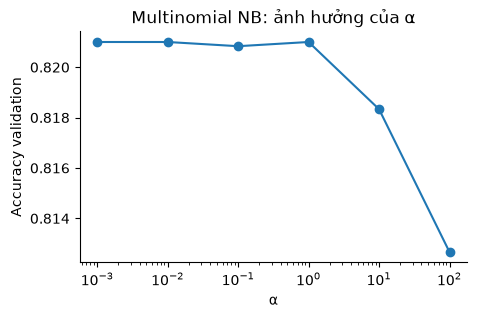
\includegraphics[width=\linewidth]{figures/nb_alpha.png}
  \caption{Multinomial NB: hệ số làm trơn $\alpha$.}\label{fig:nb_alpha}
\end{subfigure}\hspace{1.5cm}
\begin{subfigure}[b]{0.36\textwidth}\centering
  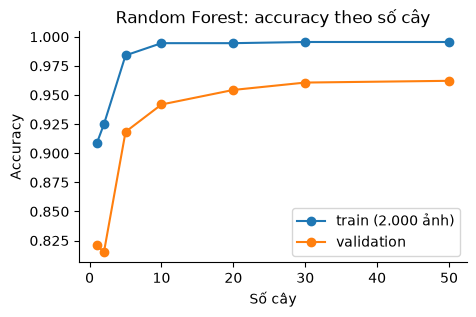
\includegraphics[width=\linewidth]{figures/rf_trees.png}
  \caption{Random Forest: accuracy theo số cây.}\label{fig:rf_trees}
\end{subfigure}\\[4pt]
\begin{subfigure}[b]{0.56\textwidth}\centering
  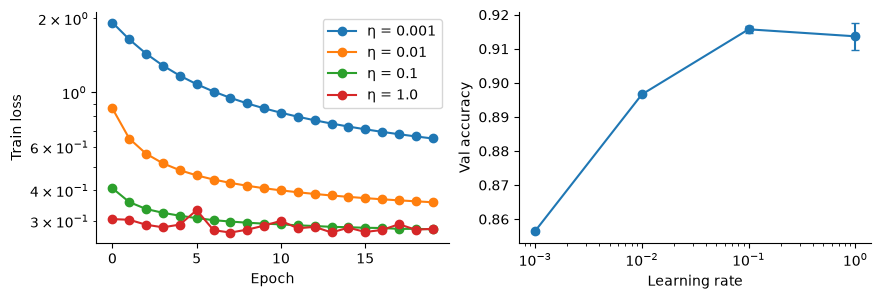
\includegraphics[width=\linewidth]{figures/lr_sweep.png}
  \caption{Logistic Regression: loss theo epoch và val accuracy theo $\eta$ (3 seed).}\label{fig:lr_sweep}
\end{subfigure}\hfill
\begin{subfigure}[b]{0.33\textwidth}\centering
  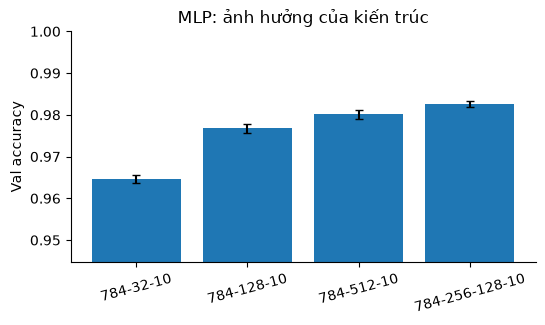
\includegraphics[width=\linewidth]{figures/mlp_arch.png}
  \caption{MLP: kiến trúc (3 seed).}\label{fig:mlp_arch}
\end{subfigure}
\caption{Accuracy validation theo siêu tham số của bốn bộ phân lớp. Thanh lỗi: độ lệch chuẩn qua 3 hạt giống.}\label{fig:hparams}
\end{figure}
 
\begin{itemize}
\item \textbf{NB (Hình~\ref{fig:nb_alpha})}: accuracy gần như phẳng ($\approx0.821$) với $\alpha\le1$, rồi giảm còn 0.818 ở $\alpha=10$ và 0.813 ở $\alpha=100$. Tổng mực mỗi lớp lên tới hàng trăm nghìn, nên $\alpha$ nhỏ hầu như không đổi $\theta$; $\alpha$ lớn kéo mọi $\theta_{cj}$ về phân phối đều, xoá đi hình dạng chữ số. Giá trị $10^{-3}$ được chọn nhưng khác biệt với $\alpha=1$ là không đáng kể.
\item \textbf{Logistic Regression (Hình~\ref{fig:lr_sweep})}: $\eta=10^{-3}$ hội tụ quá chậm (0.856 sau 20 epoch), $\eta=10^{-2}$ đạt 0.897; $\eta=0.1$ đạt cao nhất (0.916) với độ lệch nhỏ. $\eta=1$ có trung bình tương đương nhưng loss dao động mạnh theo epoch và độ lệch chuẩn giữa các seed lớn hơn, nên $\eta=0.1$ được chọn.
\item \textbf{MLP (Hình~\ref{fig:mlp_arch})}: accuracy tăng theo dung lượng mô hình: 0.965 (32 nơ-ron) $\to$ 0.977 (128) $\to$ 0.980 (512) $\to$ 0.983 (256-128). Mạng hai lớp ẩn tốt nhất dù có ít tham số hơn mạng 784-512-10 (235\,146 so với 407\,050).
\item \textbf{Random Forest (Hình~\ref{fig:rf_trees})}: một cây đạt khoảng 0.82, hai cây còn thấp hơn (soft voting của 2 cây dễ hoà), 10 cây đạt 0.94, rồi bão hoà quanh 0.96 từ 30 cây. Accuracy train (đo trên 2\,000 ảnh train) đạt $\approx$1.0 từ 10 cây: khoảng cách train--validation không thu hẹp khi thêm cây, vì thêm cây chỉ giảm phương sai chứ không giảm độ phức tạp từng cây.
\end{itemize}
 
\subsection{Confusion matrix trên tập test}
 
\begin{figure}[H]
\centering
\begin{subfigure}[b]{0.245\textwidth}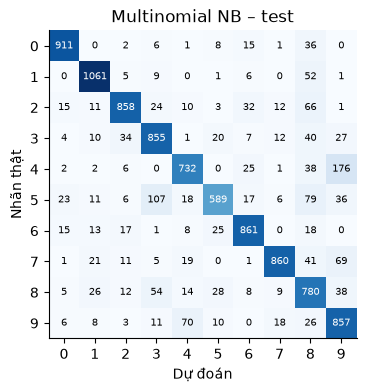
\includegraphics[width=\linewidth]{figures/cm_test_nb.png}\end{subfigure}\hfill
\begin{subfigure}[b]{0.245\textwidth}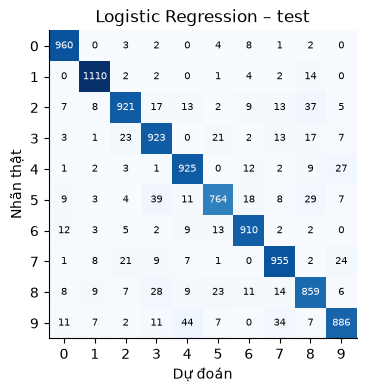
\includegraphics[width=\linewidth]{figures/cm_test_lr.png}\end{subfigure}\hfill
\begin{subfigure}[b]{0.245\textwidth}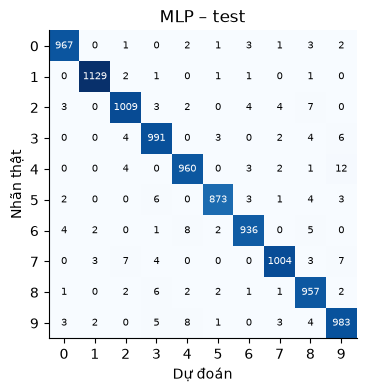
\includegraphics[width=\linewidth]{figures/cm_test_mlp.png}\end{subfigure}\hfill
\begin{subfigure}[b]{0.245\textwidth}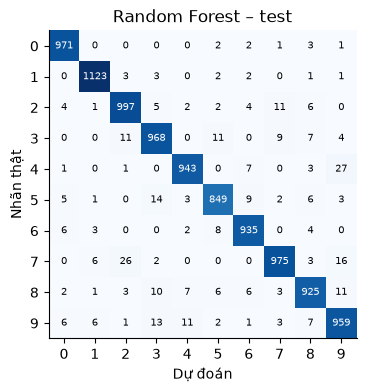
\includegraphics[width=\linewidth]{figures/cm_test_rf.png}\end{subfigure}
\caption{Confusion matrix trên 10\,000 ảnh test (hàng: nhãn thật, cột: dự đoán). Tổng số lỗi: NB 1\,636, LR 787, MLP 191, RF 355.}\label{fig:cm}
\end{figure}
 
\begin{table}[H]
\centering\small
\caption{Recall từng lớp trên tập test, tính từ Hình~\ref{fig:cm}. In đậm: lớp khó nhất của mỗi mô hình.}\label{tab:recall}
\begin{tabular}{@{}lcccccccccc@{}}
\toprule
Mô hình & 0 & 1 & 2 & 3 & 4 & 5 & 6 & 7 & 8 & 9 \\
\midrule
Multinomial NB      & 0.930 & 0.935 & 0.831 & 0.847 & 0.745 & \textbf{0.660} & 0.899 & 0.837 & 0.801 & 0.849 \\
Logistic Regression & 0.980 & 0.978 & 0.892 & 0.914 & 0.942 & \textbf{0.857} & 0.950 & 0.929 & 0.882 & 0.878 \\
MLP                 & 0.987 & 0.995 & 0.978 & 0.981 & 0.978 & 0.979 & 0.977 & 0.977 & 0.983 & \textbf{0.974} \\
Random Forest       & 0.991 & 0.989 & 0.966 & 0.958 & 0.960 & 0.952 & 0.976 & \textbf{0.948} & 0.950 & 0.950 \\
\bottomrule
\end{tabular}
\end{table}
 
\begin{table}[H]
\centering\small
\caption{Số lỗi của các cặp hay nhầm (cộng cả hai chiều, ví dụ $4\leftrightarrow9$ = $4\to9$ + $9\to4$) trên tập test.}\label{tab:pairs}
\begin{tabular}{@{}lcccccc@{}}
\toprule
Mô hình & $4\leftrightarrow9$ & $3\leftrightarrow5$ & $7\leftrightarrow9$ & $2\leftrightarrow7$ & $2\to8$ & Tổng lỗi \\
\midrule
Multinomial NB      & 246 (176+70) & 127 (20+107) & 87 & 23 & 66 & 1\,636 \\
Logistic Regression & 71 (27+44)   & 60 (21+39)   & 58 & 34 & 37 & 787 \\
MLP                 & 20 (12+8)    & 9 (3+6)      & 10 & 11 & 7  & 191 \\
Random Forest       & 38 (27+11)   & 25 (11+14)   & 19 & 37 (11+26) & 6 & 355 \\
\bottomrule
\end{tabular}
\end{table}
 
Ở cả bốn mô hình, phần lớn khối lượng nằm trên đường chéo; chữ số 0 và 1 dễ nhất (recall $\ge0.93$ ở mọi mô hình). Cặp $4\leftrightarrow9$ là nguồn lỗi chung lớn nhất. Naive Bayes có các cột ``hút'' lỗi rõ rệt: cột 8 nhận 396 ảnh sai và cột 9 nhận 348 ảnh sai; riêng chữ số 5 bị đoán thành 3 tới 107 lần, khiến recall lớp 5 chỉ 0.66.